\documentclass[a4paper,12pt]{article}
\usepackage[left=2cm,right=1cm,top=2cm,bottom=2cm]{geometry}
\usepackage{amsmath}
\usepackage{listings}
\usepackage{latexsym}
\usepackage{amsmath}
\usepackage{amssymb}
\usepackage{graphicx}
\usepackage{wrapfig}
\pagestyle{plain}
\usepackage{fancybox}
\usepackage{bm}
\usepackage[utf8]{inputenc}
\usepackage[russian]{babel}
\usepackage{floatrow}
\usepackage{pdfpages}
\usepackage{ragged2e}
\usepackage{algorithm}
\usepackage{algpseudocode}
\usepackage{listings}
\usepackage{xcolor}
\lstdefinestyle{mystyle}{
    breakatwhitespace=false,         
    breaklines=true,                 
    captionpos=b,                    
    keepspaces=true,                 
    numbers=left,                    
    numbersep=5pt,                  
    showspaces=false,                
    showstringspaces=false,
    showtabs=false,                  
    tabsize=2,
    frame=single
}
\lstset{style=mystyle}
\usepackage[T2A]{fontenc}
\usepackage[utf8]{inputenc}
\usepackage[russian, english]{babel}
\justifying
\usepackage[inkscapeformat=png]{svg}
\usepackage[pageanchor]{hyperref}
\algblock[BLOCK]{parfor}{endparfor}


\begin{document}
\tableofcontents
\hyperpage{}

\newpage
\section{Введение} 
В данной статье мы рассмотрим модифицированный метод Лагерра, который обладает важным достоинством в виде локальной сходимости четвертого порядка [1]. 

Во втором разделе мы определяем формулу модифицированного метода Лагерра для обновления приближений корня для общего случая и для случая простых корней; на основе процедуры Бини подбираем начальные приближения, которые на практике почти всегда сходятся к корням многочлена; определяем процедуру вычисления поправочного члена с учетом машинной точности; описываем численно устойчивый метод для решения квадратного уравнения, возникающее в методе Лагерра; рассматриваем критерий остановки, гарантирующий, что итерации не прекратятся до тех пор, пока полученное значение не станет надежным для приближения корня.

В третьем разделе мы поэтапно описываем работу рассматриваемого алгоритма, приводим способ реализации с помощью псевдокода.

В четвертом разделе мы приводим способ имплементации данного алгоритма с помощью языка программирования C++, описываем реализованные функции и классы.

В пятом разделе мы демонстрируем результаты проведенных тестов для полиномов различных степеней.


\newpage
\section{Теоретическое обоснование}
\subsection{Вывод метода}

Рассмотрим полином $p$ от переменной $z$, определенный следующим образом:
\[p(z) = a_0 + a_{1}z + \text{···} + a^{m}z^{m} \eqno (1) \]
где $a_0a_m \neq 0$. Если $a_0 = 0$, полином делится на линейный коэффициет и метод применяется к полученному полиному. Обозначим \{$z_1, \text{...}, z_m$\} текущее приближение к корням \{$\zeta_1, \text{...}, \zeta_m$\} полинома $p$. Суть алгоритма заключается в обновлении каждого приближения $z_j$, пока оно не станет "достаточно близким" \: к корню $\zeta_j$.

Метод Лагерра выполняет это обновление, решая квадратное уравнение, которое мы обозначим $Q_j(z)=0$.Отметим, что если корни $p$ вещественные, то оба решения  $Q_j(z)=0$ будут гарантированно ближе к $\zeta_j$, чем текущее приближение $z_j$. Именно этим объясняется глобальная сходимость метода Лагерра, когда корни полинома вещественные. 

Обозначим корни уравнения $Q_j(z)$ с помощью $\hat{z}_j$ и отметим, что:
\[ \hat{z}_j = z_j - \frac{m}{G_j \pm \sqrt{(m-1)(mH_j-G^{2}_{j})}} \eqno (2) \]
где
\[ G_j=\frac{p'(z_j)}{p(z_j)}=\displaystyle\sum_{i=1}^{m} \frac{1}{(z_i-\zeta_i)} \qquad H_j=-\left(\frac{p'(z_j)}{p(z_j)}\right)'=\displaystyle\sum_{i=1}^{m} \frac{1}{(z_i-\zeta_i)^2} \eqno (3) \]
Обновление $z_j$ определеятся ближайшим $\hat{z}_j$; то есть мы выбираем знак, который максимизирует знаменатель дроби в $(2)$. Назовем это обновление \textit{поправочным членом} $z_j$.

Для случая с простыми корнями, уравнение $(3)$ записывается в виде невязки:
\[ \hat{G_j}=\frac{p'(z_j)}{p(z_j)}-\displaystyle\sum_{\substack{i=1 \\ i \neq j}}^{m} \frac{1}{(z_j-z_i)} 
\qquad 
\hat{H_j}=-\left(\frac{p'(z_j)}{p(z_j)}\right)'-\displaystyle\sum_{\substack{i=1 \\ i \neq j}}^{m} \frac{1}{(z_j-z_i)^2}  
\eqno (4) \]
Более того, это эквивалентно применению метода Лагерра к функции
\[ f_j(z)=\frac{p(z)}{\prod_{\substack{i=1 \\ i \neq j}}^{m}(z_j-z_i)} \eqno (5) \]
при вычислении поправочного члена $z_j$. Таким образом, мы создаем полюса во всех других корневых аппроксимациях и, следовательно, избегаем ненужной множественной сходимости к одному и тому же корню.

\newpage
\subsection{Начальная аппроксимация}
Как и во всех итерационных методах, производительность модифицированного метода Лагерра существенно зависит от качества начальных приближений. Для их вычисления будет применяться процедура, предложенная Бини [2], которая выбирает комплексные числа вдоль окружностей подходящих радиусов, которые можно формализировать применив теорему Пелле [3].

\bigskip
\textit{Теорема $1.$} Пусть $p$ - полином, определенный в $(1)$. Для каждого $k$, такого что $a_k \neq 0$, рассмотрим уравнение:
\[ |a_k|z^k = \displaystyle\sum_{\substack{i=0 \\ i \neq k}}^{m} |a_i|z^i \eqno (6) \]

\begin{enumerate}
    \item Если $k=0$, существует одно положительное вещественное решение $s_0$, и $p$ не имеет корней, которые по модулю меньше, чем $s_0$.
    \item Если $0 < k < m$, то вещественных положительных решений либо нет, либо есть два вещественных положительных решения $t_k \leq s_k$. В последнем случае $p$ не имеет корней в открытом кольце $A(t_k, s_k)$ и ровно $k$ корней с модулями меньшими или равными $t_k$.
    \item Если $k = m$, существует одно положительное решение $t_m$, и $p$ не имеет корней с модулями больше, чем $t_m$.  
\end{enumerate}

Пусть $0 = k_1 < k_2 < \text{...} < k_q = m$ - значения $k$, для которых в $(6)$ существует позитивное(-ые) решение(-я), тогда пусть
$$s_0 = s_{k_1} \leq t_{k_2} \leq s_{k_2} \leq \text{...} \leq t_{k_{q-1}} \leq t_{k_q} = t_m$$
- эти решения. Тогда, каждый полином в классе 
$$\mathcal P(p)= \left\{ \displaystyle\sum_{i=0}b_i z^i: |b_i|=|a_i|\right\}$$
имеет $(k_{i+1}-k_i)$ нулей в замкнутом кольце $\bar{\mathcal A}(t_{k_i},s_{k_i})$, для $i=1,\text{...},q-1,$ и ни одного нуля в открытом кольце $\mathcal A(t_{k_i},s_{k_i})$, для $i=1,\text{...},q$.

Хотя эти данные могут быть использованы для определения начальных приближений нашего итерационного метода, формирование положительных решений $(6)$ требует решения нескольких полиномиальных уравнений. Поэтому мы ищем стратегию с наименьшей временной сложностью. Для этого определим:
\begin{equation}
\begin{split}
    u_k &=\max_{i < k} \left| \frac{a_i}{a_k}\right|^{1/(k-i)}, k = 1, \text{...}, m,\\
    v_k &=\min_{\substack{i > k \\ a_i \neq 0}} \left| \frac{a_i}{a_k}\right|^{1/(k-i)}, k = 0, \text{...}, m-1, \\
    u_0 &= 1/(1 + \max_{i>0}\left| \frac{a_i}{a_0}\right|) \\
    v_0 &= 1 + \max_{i<m}\left| \frac{a_i}{a_0}\right|.
\end{split}
\tag{7}
\end{equation}

Тогда, получаем, что положительные решения $(6)$ удовлетворяют
\[ u_{k_i} \leq t_{k_i} \leq s_{k_i} \leq v_{k_i}, i = 1, \text{...}, q. \eqno (8) \]

Рассмотрим множество $\mathcal{C}=\{(i, \log|a_i|), i=0,1,\text{...}, m\}$ и обозначим $$\gamma(\mathcal{C}) = \{(\hat{k}_i, \log|a_{\hat{k}_i}|), 0=\hat{k}_1<\hat{k}_2<\text{...}<\hat{k}_{\hat{q}}=m\}$$
верхняя огибающая выпуклой оболочки $\mathcal{C}$. Мы знаем, что вершины $\gamma(\mathcal{C})$ удовлетворяют условиям $u_l \leq v_l$ тогда и только тогда, когда $l \in \{\hat{k}_1,\text{...},\hat{k}_{\hat{q}}\}$. Следовательно, согласно $(8)$, имеем $\{k_1,\text{...},k_q\} \subseteq \{\hat{k}_1,\text{...},\hat{k}_{\hat{q}}\}$, где содержащее множество может быть вычислено эффективно. Поскольку множество $\mathcal{C}$ упорядочено относительно первый координаты, целесообразно будет использовать алгоритм монотонный цепочки Эндрю для вычисления $\gamma(\mathcal{C})$, который в данном случае имеет временную сложность $O(m)$.

\newpage 
\subsection{Алгоритм Эндрю} 
\textbf{Алгоритм Эндрю} - алгоритм построения выпуклой оболочки в двумерном пространстве, является модификацией алгоритма Грэхема. 

\textbf{Выпуклой оболочкой} множества $S$ называется наименьшее выпуклое множество (множество, в котором все точки отрезка, образуемого любыми двумя точками данного множества, также принадлежат данному множеству), содержащее $S$.

\begin{figure}[H]
\vspace{-0.5em}
\captionsetup{justification=centering, skip=-0.5em}
  \centering
  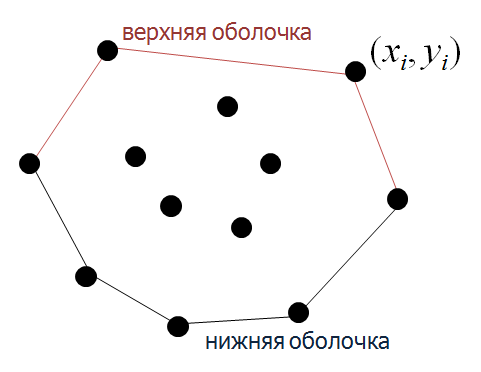
\includegraphics[width=0.5\textwidth]{images/convex_hull.png}
  \caption{Пример выпуклой оболочки для набора точек}
\vspace{-1em}
\end{figure}

Сначала алгоритм сортирует набор точек $S$ по возрастанию координаты $x$, а затем $y$. Пусть минимальные и максимальные координаты $x$ будут $x_{\min}$ и $x_{\max}$. Очевидно что у первой из точек $x=x_{\min}$, а у последней $x=x_{\max}$. Cоединим эти две точки отрезком. Остальное множество точек разделяется на два, в зависимости от того, с какой стороны от этой прямой точки лежат. Таким образом, мы можем определить новую нижнюю и новую верхнюю линии. В совокупности эти линии и дают требуемую оболочку.

Для построения верхней оболочки точки множества $S$ упорядочивается в соответствии с возрастанием абсциссы и после совершается работа полученных данных по алгоритму Грэхема (см. раздел №3). Для этого алгоритм Эндрю использует стек $x_0, x_1, \dots, x_t$ для хранения текущей верхней оболочки. Точка $x_t$ считается находящейся на вершине стека. После окончания работы алгоритма стек содержит верхнюю оболочку множества $S$.

\newpage
\subsection{Вычисление поправочного члена}
В данном разделе мы рассматриваем численно устойчивый метод вычисления поправочного члена $\hat{z_{j}}$ (2), который используется для обновления приближения корня $z_j$.
\\
Пусть $fl(p(\xi))$ представляет собой вычисленное значение функции $p$, оцененное в  $\xi \in \mathbb{C}$ с использованием арифметики с плавающей точкой и машинной точностью $\mu$. 
Тогда, используя метод Руффини-Хорнера получаем:
\[  fl(p(\xi)) = \sum_{i=0}^{m} a_i(1 + \epsilon_{i})\xi^i \eqno (9)\], где $|\epsilon_i| < ((2\sqrt{2} + 1)i + 1)\mu + O(\mu^2)$
Аналогичный результат имеет место быть для первой и второй производной
\\
Метод Руффини-Хорнера склонен к переполнению при больших степенях полинома с положительными коэффициентами в точке $\xi$, где $|\xi| > 1$. По этой причине мы вводим обратный полином, определяемый как:
\[p_{R}(z) = a_{0}z^m + ... + a_{m - 1}z+a_{m} \eqno (10)\]
\\
Если $z \neq 0$, то $\rho = \frac{1}{z}$. Получаем соотношения:
\begin{equation}
\begin{aligned}
\frac{p^{\prime}(z)}{p(z)} &= \rho\left(m - \rho\frac{p^{\prime}_{R}(\rho)}{p_{R}(\rho)}\right) , \\
-\left(\frac{p^{\prime}(z)}{p(z)}\right)^{\prime} &= \rho^2\left(m - 2\rho\frac{p^{\prime}_R(\rho)}{p_R(\rho)} - \rho^2\left(\frac{p^{\prime}_{R}(\rho)}{p_R(\rho)}\right)^{\prime}\right)
\end{aligned}
\tag{11}
\end{equation}

Оценим временную сложность нашего алгоритма: начальные приближения в Алгоритме 1 вычисляются за время $O(m)$, затем каждое приближение обновляется за $O(m)$ следуя методу Руффини-Хорнера. Выходит, что Алгоритм 3 при фиксированном коэффициенте аппроксимирует все корни многочлена за $O(m^2)$
\newpage
\subsection{Критерий остановки}
Пусть $\xi$ - аппроксимация корня $\zeta$, где все вычисления имеют машинную точность $\mu$. В данном разделе мы вычислим обратную ошибку, которая измеряет то, насколько сильно нужно изменить коэффициенты многочлена, чтобы приближенный корень стал точным. Если обратная ошибка меньше или равна машинной точности, то алгоритм прекращает итерации и возвращает приближенный корень и его число обусловленности,где число обусловленности измеряет, насколько сильно изменение коэффициентов многочлена влияет на изменение корня. Если обратная ошибка больше машинной точности, то алгоритм продолжает итерации, пока не будет достигнут критерий остановки или не будет превышено максимальное число итераций.
\\
Естественное определение обратной ошибки $\xi$ выглядит следующим образом:
\[\eta(\xi) = min\{\epsilon: (p+\Delta p)(\xi) = 0, |\Delta a_i| \leq \epsilon|e_i|, i=0, 1,..., m\}, \eqno (12) \] где
\[\Delta p(z) = \Delta a_0 + \Delta a_1z+...+\Delta a_m z^m \eqno (13)\]
Обратную ошибку можно определить как:
\[\eta(\xi) = \frac{p(\xi)}{\alpha(\xi)},\text{     } \alpha(\xi) = \sum_{i = 0}^{m}|e_i||\xi|^i  \eqno (14)\]
Исходя из анализа обратных ошибок правила Руффини-Хорнера (2.3), положим $e_i = ((2\sqrt{2} + 1)i + 1)a_i$. Тогда если $\eta(\xi) \leq \mu$, то $\xi$ это корень $(p + \Delta p)$ и коэффициенты $\Delta a_i$ не больше чем $\epsilon_i$. Таким образом этот критерий остановки гарантирует, что итерации не прекратятся до тех пор, пока $fl(p(\xi)$ не перестанет быть надежным для приближения корня $\xi$.
\\
Из секции вычисления поправочного члена, если $|\xi| > 1$, то мы работаем с обратным полиномом. Тогда обратная ошибка вычисляется как:
\[\eta(\xi) = \frac{|p_R(\rho)|}{\alpha_R(\rho)}, где \alpha_R(\rho) = \sum_{i = 0}^{m} |e_{m - i}||\rho|^i  \eqno (15)\]
Число обусловленности корня:
\[\kappa(\xi, \rho) = \frac{\alpha(\xi)}{|\xi||p'(\xi)|} \eqno (16)\]
В итоге мы возвращаем значения $\kappa$ и $\eta$, которые используются как критерий остановки и примерная чувствительность $\zeta$ к изменениям коэффициентов p. Произведение же $\eta(\xi)\kappa(\zeta, p)$ используется для получения ограничения первого порядка на ошибку прямого хода в приближении $\xi$.


\newpage
\section{Описание работы алгоритма}
Пусть $p(z)$ - полином следующего вида:
$$p(z) = a_0 + a_{1}z + \text{···} + a_{m}z^{m}$$
Мы стремимися вычислить корни $p(z)$ и для этого необходимо выполнить следующие пункты:
\begin{enumerate}
    \item Найти начальное приближение:
        \begin{algorithm}
            \caption{Вычисление начального приближения}\label{alg:Example}
            \begin{algorithmic}
            \State \text{Вычислить} $\hat{k}_1,\text{...}, \hat{k}_{\hat{q}}$ \text{с помощью алгоритма монотонной цепи Эндрю} 
            \For{$i=1$ to $\hat{q}-1$}
                \State $n=\hat{k}_{i+1}-\hat{k}_i$
                \State $u_{\hat{k_{i+1}}}=\left| \frac{a_{\hat{k}_i}}{a_{\hat{k}_{i+1}}} \right|^{1/n}$
                \For{$j=1$ to $n$}
                    \State $z_{\hat{k}_{i} + i} = u_{\hat{k}_{i+1}}e^{\left(\frac{2\pi}{n}j + \frac{2\pi}{m} + \sigma\right)i}$
                \EndFor
            \EndFor 
            \end{algorithmic}
        \end{algorithm}

        Для вычисления $\hat{k}_1,\text{...}, \hat{k}_{\hat{q}}$ используется следующий алгоритм:
        \begin{algorithm}[H]
            \caption{Алгоритм Эндрю для нахождения верхней оболочки}\label{alg:Example}
            \begin{algorithmic}
            \State \text{Функция определения направления поворота для трех точек:}
            \Function{cross}{Point p, Point q, Point r}
                \State val = (r.x - q.x) * (q.y - p.y)  - (q.x - p.x) * (r.y - q.y)
                \If{val = 0}
                    \State return 0
                \ElsIf{val > 0}
                    \State return 1
                \Else
                    \State return 2
                \EndIf
            \EndFunction
            \State
            \State $P\gets \text{список из $m$ точек в двумерной плоскости}$
            \State \text{Отсортировать точки P по x-координате (в случае совпадения сортировка по y-координате)}
            \For{$i=m$ to $1$}
                \State $\text{p = P[i]}$
                \State $\text{L\_upper} \gets \text{верхняя оболочка}$
                \State \text{top возвращает верхнюю точку в стеке}
                \State \text{nextToTop возвращает вторую сверху точку в стеке}
                \While{len(L\_upper) >= 2 and cross(nextToTop(L\_upper), top(L\_upper), p) != 2}
                    \State L\_upper.pop()
                \EndWhile
                \State L\_upper.append(p)
            \EndFor
            \end{algorithmic}
        \end{algorithm}



    \item Обновлять начальное приближение, пока оно не станет "достаточно близко"\ к корням полинома, или пока не пройдет определенное число итераций.
            \begin{algorithm}[H]
                \caption{Нахождение корней полинома}\label{alg:Example}
                \begin{algorithmic}
                \State $(z_1, \text{...}, z_m)\gets\text{Начальная аппроксимация полученная с помощью Алгоритма 1}$
                \While{$i < $ \text{itmax}}
                    \For{$j=1$ to $m$}
                        \If{$z_j$ недостаточно близок к $\zeta_j$}
                            \State Вычислить корни $Q_j(\lambda)$ с помощью $(2)$, используя $(4)$
                            \State $z_j \gets \text{корень, который максимизирует знаменатель в } (2)$
                        \EndIf
                    \EndFor
                    \State $i \gets i+1$
                \EndWhile
                \end{algorithmic}
            \end{algorithm}     
\end{enumerate}


\clearpage
\newpage
\section{Имплементация на C++}

\subsection{ExtendedFunctions.h}
\textbf{Описание:}

Набор необходимых функций для реализации алгоритмов нахождения корней полиномов.

\textbf{Функции:}
\begin{itemize}
    \item \textbf{anynotfinite (bool)} : проверка, является ли хотя бы одно число не конечным;
    \\Аргументы функции:
    \begin{itemize}
        \renewcommand{\labelitemi}{-}
        \item \textbf{T \&\& ... t } : множество чисел (любое количество).
    \end{itemize}
    \begin{lstlisting}[language=С++]
inline bool anynotfinite(T && ... t); \end{lstlisting}

    \item \textbf{complexnotfinite (bool)} : проверка, содержит ли комплексное число значения NaN или Inf;
    \\Аргументы функции:
    \begin{itemize}
        \renewcommand{\labelitemi}{-}
        \item \textbf{a (complex<T>)} : комплексное число;
        \item \textbf{big (T)} : максимальное значение для типа T.
    \end{itemize}
    \begin{lstlisting}[language=С++]
bool complexnotfinite(complex<T> a, T big); \end{lstlisting}

    \item \textbf{anycomplex (bool)} : проверка, что хотя бы одно комплесное число содержит мнимую часть;
    \\Аргументы функции:
    \begin{itemize}
        \renewcommand{\labelitemi}{-}
        \item \textbf{T \&\& ... t } : множество чисел (любое количество).
    \end{itemize}
    \begin{lstlisting}[language=С++]
inline bool anycomplex(T && ... t); \end{lstlisting}

    \item \textbf{anycomplex (bool)} : проверка, что хотя бы одно комплесное число в векторе содержит мнимую часть;
    \\Аргументы функции:
    \begin{itemize}
        \renewcommand{\labelitemi}{-}
        \item \textbf{vec (vector<complex<T>>)} : вектор комплексных чисел.
    \end{itemize}
    \begin{lstlisting}[language=С++]
inline bool anycomplex(vector<complex<T>> vec); \end{lstlisting}

    \item \textbf{sign (int)} : определение знака числа
    \\Аргументы функции:
    \begin{itemize}
        \renewcommand{\labelitemi}{-}
        \item \textbf{val (number)} : заданное значение;
    \end{itemize}

    Возвращаемое значение: если заданное значение положительно, функция возвращает 1, если отрицательно, возвращает -1, если значение равно 0, возвращает 0.

    \begin{lstlisting}[language=С++]
inline int sign(number val); \end{lstlisting}

    \item \textbf{fms (number)} : операция "fused multiply-subtract" (FMS), которая вычисляет разность произведения первых двух чисел и других двух чисел;
    \\Аргументы функции:
    \begin{itemize}
        \renewcommand{\labelitemi}{-}
        \item \textbf{a (number)} : первое число;
        \item \textbf{b (number)} : второе число;
        \item \textbf{c (number)} : третье число;
        \item \textbf{d (number)} : четвертое число;
    \end{itemize}
    Возвращаемое значение: число $a\cdot b - d \cdot c$.

    \begin{lstlisting}[language=С++]
inline number fms(number a, number b, number c, number d); \end{lstlisting}

    \item \textbf{fms (complex<number>)} : операция "fused multiply-subtract" (FMS) для комплесных чисел, которая вычисляет разность произведения первых двух чисел и других двух чисел;
    \\Аргументы функции:
    \begin{itemize}
        \renewcommand{\labelitemi}{-}
        \item \textbf{a (std::complex<number>)} : первое комплесное число;
        \item \textbf{b (std::complex<number>)} : второе комплесное число;
        \item \textbf{c (std::complex<number>)} : третье комплесное число;
        \item \textbf{d (std::complex<number>)} : четвертое комплесное число;
    \end{itemize}
    Возвращаемое значение: комплесное число $a\cdot b - d \cdot c$.
    \begin{lstlisting}[language=С++]
inline complex<number> fms(std::complex<number> a, 
                        std::complex<number> b, 
                        std::complex<number> c,
                        std::complex<number> d); \end{lstlisting}


    \item \textbf{fma (complex<number>)} : операция "fused multiply-add" (FMA) для комплесных чисел, которая вычисляет разность произведения двух чисел и третьего числа;
    \\Аргументы функции:
    \begin{itemize}
        \renewcommand{\labelitemi}{-}
        \item \textbf{a (std::complex<number>)} : первое комплесное число;
        \item \textbf{b (std::complex<number>)} : второе комплесное число;
        \item \textbf{c (std::complex<number>)} : третье комплесное число;
    \end{itemize}
    Возвращаемое значение: комплесное число $a\cdot b - c$.
    \begin{lstlisting}[language=С++]
inline complex<number> fma(std::complex<number> a, 
                        std::complex<number> b, 
                        std::complex<number> c); \end{lstlisting}

    \item \textbf{printVec (void)} : вывод вектора чисел в консоль;
    \\Аргументы функции:
    \begin{itemize}
        \renewcommand{\labelitemi}{-}
        \item \textbf{vec (vector<number>)} : вектор чисел;
    \end{itemize}
    \begin{lstlisting}[language=С++]
inline void printVec(vector<number> vec); \end{lstlisting}

    \item \textbf{castVec (vector<number>)} : преобразование вектора с типом T в вектор с типом number;
    \\Аргументы функции:
    \begin{itemize}
        \renewcommand{\labelitemi}{-}
        \item \textbf{vec (vector<T>)} : вектор чисел;
    \end{itemize}
    Возвращаемое значение: вектор чисел типа number.
    \begin{lstlisting}[language=С++]
inline vector<number> castVec(vector<T> vec); \end{lstlisting}
\end{itemize}



\subsection{Класс BaseSolver}
\textbf{Описание класса:}

Абстрактный базовый класс для нахождения корней полиномов. 

\textbf{Методы класса:}
\begin{itemize}
    \item \textbf{operator() (void)} : нахождение корней полинома;

\\Аргументы метода:
    \begin{itemize}
        \renewcommand{\labelitemi}{-}
        \item \textbf{coeff (std::vector<T>\&)} : вектор, содержащий коэффициенты полинома;
        \item \textbf{roots (std::vector<std::complex<T>\& )} : вектор для хранения корней полинома;
        \item \textbf{conv (std::vector<int>\&)} : вектор для хранения статуса сходимости каждого корня;
        \item \textbf{itmax (int)} : максимально допустимое количество итераций.
    \end{itemize}
\begin{lstlisting}[language=С++]
virtual void operator()(std::vector<T>& coeff, 
                        std::vector<std::complex<T>>& roots, 
                        std::vector<int>& conv, 
                        int itmax) = 0; \end{lstlisting}
\end{itemize}
    
\subsection{Класс ModifiedLaguerre18}
\textbf{Описание класса:}

Класс, реализующий модифицированный алгоритм Лагерра для поиска корней полинома, основанный на статье [4].

\textbf{Атрибуты класса:}
\begin{itemize}
\renewcommand{\labelitemi}{-}
    \item \textbf{eps (T)} : машинная точность для типа T;
    \item \textbf{big (T)} : максимальное значение для типа T;
    \item \textbf{small (T)} : минимальное положительное значение для типа T;
    \item \textbf{PI (T)} : значение числа Пи для типа T;
    \item \textbf{pi2 (T)} : удвоенное значение числа Пи для типа T.
\end{itemize}

\textbf{Методы класса:}
\begin{itemize}
    \item \textbf{ModifiedLaguerre18()} : конструктор класса \textbf{ModifiedLaguerre18};
    
    \item \textbf{operator() (void)} : нахождение корней полинома с использованием модифицированного метода Лагерра;
    \\Аргументы метода:
    \begin{itemize}
        \renewcommand{\labelitemi}{-}
        \item \textbf{poly (std::vector<T>\&)} : вектор, содержащий коэффициенты полинома;
        \item \textbf{roots (std::vector<std::complex<T>\& )} : вектор для хранения корней полинома;
        \item \textbf{conv (std::vector<int>\&)} : вектор для хранения статуса сходимости каждого корня;
        \item \textbf{itmax (int)} : максимально допустимое количество итераций.
    \end{itemize}
    \begin{lstlisting}[language=С++]
void operator()(std::vector<T>& poly, 
                std::vector<std::complex<T>>& roots, 
                std::vector<int>& conv, int itmax); \end{lstlisting}

    \item \textbf{cross (T)} : нахождение величины кросс-произведения (векторного произведения) двух векторов;
    \\Аргументы метода:
    \begin{itemize}
        \renewcommand{\labelitemi}{-}
        \item \textbf{h (std::vector<int>\&))} : вектор целых чисел, представляющих точки;
        \item \textbf{a (std::vector<T>\&)} : вектор значений типа T, представляющих координаты точек;
        \item \textbf{c (int)} : индекс текущей точки;
        \item \textbf{i (int)} : Индекс следующей точки.
    \end{itemize}
    
    Возвращаемое значение: величина кросс-произведения заданных векторов (T)

        \begin{lstlisting}[language=С++]
inline T cross(std::vector<int>& h, 
            std::vector<T>& a, 
            int c, 
            int i); \end{lstlisting}

    \item \textbf{conv\_hull (void)} : нахождение выпуклой оболочки заданного набора точек;
    \\Аргументы метода:
    \begin{itemize}
        \renewcommand{\labelitemi}{-}
        \item \textbf{n (int)} : количество точек;
        \item \textbf{a (std::vector<T>\&)} : вектор значений типа T, представляющих координаты точек;
        \item \textbf{h (std::vector<int>\&)} : вектор для хранения выпуклой оболочки;
        \item \textbf{c (int\&)} : количество точек в выпуклой оболочке.
    \end{itemize}
    \begin{lstlisting}[language=С++]
inline void conv_hull(int n, 
                    std::vector<T>& a, 
                    std::vector<int>& h, 
                    int& c); \end{lstlisting}

    \item \textbf{estimates (void)} : оценка корней полинома;
    \\Аргументы метода:
    \begin{itemize}
        \renewcommand{\labelitemi}{-}
        \item \textbf{alpha (vector<T>\&)} : вектор модулей коэффициентов полинома;
        \item \textbf{deg (int)} : степень полинома;
        \item \textbf{conv (std::vector<int>\&)} : вектор для хранения статуса сходимости каждого корня;
        \item \textbf{nz (int\&)} : количество нулей.
    \end{itemize}
    \begin{lstlisting}[language=С++]
inline void estimates(vector<T>& alpha, 
                    int deg, 
                    std::vector<std::complex<T>>& roots, 
                    std::vector<int>& conv, 
                    int& nz); \end{lstlisting}

    \item \textbf{rcheck\_lag (void)} : коррекция метода Лагерра, вычисляет обратную ошибку и проверяет условие сходимости, если модуль корня больше 1;
    \\Аргументы метода:
    \begin{itemize}
        \renewcommand{\labelitemi}{-}
        \item \textbf{p (std::vector<T>\&))} : вектор коэффициентов полинома;
        \item \textbf{alpha (vector<T>\&)} : вектор модулей коэффициентов полинома;
        \item \textbf{deg (int)} : степень полинома;
        \item \textbf{b (complex<T>\&)} : выходное комплексное число, представляющее корень;
        \item \textbf{c (complex<T>\&)} : выходное комплексное число, представляющее коррекцию;
        \item \textbf{z (complex<T>)} : комплексное число, используемое для коррекции;
        \item \textbf{r (T)} : значение, используемое для коррекции;
        \item \textbf{conv (int\&)} : выходное значение, указывающее статус сходимости;
        \item \textbf{berr (T\&)} : выходная обратная ошибка;
        \item \textbf{cond (T\&)} : выходное число условия.
    \end{itemize}

\begin{lstlisting}[language=С++]
inline void rcheck_lag(std::vector<T>& p, 
                    vector<T>& alpha, 
                    int deg, complex<T>& b, 
                    complex<T>& c, 
                    complex<T> z, 
                    T r, 
                    int& conv, 
                    T& berr, 
                    T& cond); \end{lstlisting}
    

    \item \textbf{check\_lag (void)} : коррекция метода Лагерра, вычисляет обратную ошибку и проверяет условие сходимости, если модуль корня меньше 1;
    \\Аргументы метода:
    \begin{itemize}
        \renewcommand{\labelitemi}{-}
        \item \textbf{p (std::vector<T>\&))} : вектор коэффициентов полинома;
        \item \textbf{alpha (vector<T>\&)} : вектор модулей коэффициентов полинома;
        \item \textbf{deg (int)} : степень полинома;
        \item \textbf{b (complex<T>\&)} : выходное комплексное число, представляющее корень;
        \item \textbf{c (complex<T>\&)} : выходное комплексное число, представляющее коррекцию;
        \item \textbf{z (complex<T>)} : комплексное число, используемое для коррекции;
        \item \textbf{r (T)} : значение, используемое для коррекции;
        \item \textbf{conv (int\&)} : выходное значение, указывающее статус сходимости;
        \item \textbf{berr (T\&)} : выходная обратная ошибка;
        \item \textbf{cond (T\&)} : выходное число условия.
    \end{itemize}
\begin{lstlisting}[language=С++]
inline void check_lag(std::vector<T>& p, 
                    vector<T>& alpha, 
                    int deg, complex<T>& b, 
                    complex<T>& c, 
                    complex<T> z, 
                    T r, 
                    int& conv, 
                    T& berr, 
                    T& cond); \end{lstlisting}

    \item \textbf{modify\_lag (void)} : модифицированная коррекция метода Лагерра на основе метода Аберта;
    \\Аргументы метода:
    \begin{itemize}
        \renewcommand{\labelitemi}{-}
        \item \textbf{deg (int)} : степень полинома;
        \item \textbf{b (complex<T>\&)} : выходное комплексное число, представляющее корень;
        \item \textbf{c (complex<T>\&)} : выходное комплексное число, представляющее коррекцию;
        \item \textbf{z (complex<T>)} : комплексное число, используемое для коррекции;
        \item \textbf{j (int)} : индекс корня для модификации;
        \item \textbf{roots (std::vector<std::complex<T>>\& )} : вектор оцененных корней.
    \end{itemize}
\begin{lstlisting}[language=С++]
void modify_lag(int deg, 
            std::complex<T>& b, 
            std::complex<T>& c, 
            std::complex<T> z, 
            int j, 
            std::vector<std::complex<T>>& roots); \end{lstlisting}
    
\end{itemize}

\newpage
\section{Тестирование}
Во время тестирования для каждой степени полинома случайным образом генерировалось 10000 экспериментальных полиномов. Для данных типа float рассматривались только полиномы 5-ой степени и ниже, так как при более высоких степенях происходила потеря точности коэффициентов и, как следствие, нахождение неверных корней.

\subsection{Результаты тестов для обычных корней (float)}
\begin{center}
  \begin{tabular}{|p{4.5cm}|p{5.5cm}|p{5.5cm}|}
  \hline
  \textbf{Степень полинома}  &  \textbf{Худшая абсолютная погрешность} & \textbf{Худшая относительная погрешность} \\
  \hline
  3 & 0.000259757 & 0.000380564 \\
  \hline
  4 & 0.00363469 & 0.0047001 \\
  \hline
  5 & 0.0111473 & 0.0133276 \\
  \hline
\end{tabular}
\label{tab:my_label_2}
\end{center}


\subsection{Результаты тестов для обычных корней (double)}
\begin{center}
  \begin{tabular}{|p{4.0cm}|p{4.0cm}|p{4.0cm}|p{3.0cm}|}
  \hline
  \textbf{Степень полинома}  &  \textbf{Худшая абсолютная погрешность} & \textbf{Худшая относительная погрешность} & \textbf{Диапазон корней}\\
  \hline
  5 & 0.0000004997 & 0.0000067689 & [-1, 1]\\
  \hline
  10 & 0.0000005910 & 0.0001649274 & [-1, 1]\\
  \hline
  20 & 0.0008829461 & 0.0000007432 & [-1, 1] \\
  \hline
  50 & 0.01132795287 & 0.0756564119 & [-1, 1] \\
  \hline
  100 & 0.0528136577 & 0.0538916389 & [-1, 1] \\
  \hline
  200 & 0.0930998252 & 0.0534754074 & [-1, 1] \\
  \hline
  500 & 3.5390033426 & 0.5439278577 & [-10, 10] \\
  \hline
  1000 & 67.4228850912 & 0.804489235 & [-100, 100] \\
  \hline
  2000 & 78.1241004113 & 0.85875 & [-100, 100] \\
  \hline
  5000 & 38.5979819615 & 0.876262012 & [-200, 200] \\
  \hline
  10000 & 59.8129892316 & 1.2473010413 & [-200, 200] \\
  \hline
\end{tabular}
\label{tab:my_label_2}
\end{center}

\subsection{Результаты тестов для кластеризованных корней (float)}
\begin{center}
  \begin{tabular}{|p{3.0cm}|p{3.0cm}|p{3.0cm}|p{3.0cm}|p{3.0cm}|}
  \hline
  \textbf{Степень полинома}  &  \textbf{Худшая абсолютная погрешность} & \textbf{Худшая относительная погрешность}  & \textbf{Диапазон корней} & \textbf{Максимальная разница между корнями}\\
  \hline
  3 & 0.00162196 & 0.0311852  & [-1, 1] & 1e-5\\
  \hline
  4 & 0.0155236 & 0.0176819 & [-1, 1] & 1e-5\\
  \hline
  5 & 0.00782436 & 0.0113724 & [-1, 1] & 1e-5\\
  \hline
\end{tabular}
\label{tab:my_label_2}
\end{center}

\subsection{Результаты тестов для кластеризованных корней (double)}
\begin{center}
  \begin{tabular}{|p{3.0cm}|p{3.0cm}|p{3.0cm}|p{3.0cm}|p{3.0cm}|}
  \hline
  \textbf{Степень полинома}  &  \textbf{Худшая абсолютная погрешность} & \textbf{Худшая относительная погрешность} & \textbf{Диапазон корней} & \textbf{Максимальная разница между корнями}\\
  \hline
  5 & 0.0003858524 & 0.0008009150 & [-1, 1] & 1e-5\\
  \hline
  10 & 0.002589944 & 0.0064761389 & [-1, 1] & 1e-5\\
  \hline
  20 & 0.0015857997 & 0.007432 & [-1, 1] & 1e-5\\
  \hline
  50 & 0.2114560494 & 0.1142833161 & [-1, 1] & 1e-5\\
  \hline
  100 & 0.3114560494 & 0.6281456165 & [-2, 2] & 1e-5\\
  \hline
  200 & 5.5913219644 & 0.1824598485 & [-50, 50] & 0.1\\
  \hline
  500 & 127.5988266699 & 0.9970928925 & [-100, 100] & 0.1\\
  \hline
  1000 & 404.5289142849 & 2.804489235 & [-500, 500] & 0.1\\
  \hline
  2000 & 430.6675218712 & 3.012456 & [-500, 500] & 0.1\\
  \hline
  5000 & 455.5979819615 & 3.20685 & [-500, 500] & 0.1\\
  \hline
  10000 & 489.8129892316] & 3.45474 & [-500, 500] & 0.1\\
  \hline
\end{tabular}
\label{tab:my_label_2}
\end{center}

\newpage
\section{Список литературы}
\begin{enumerate}
    \item Petkovic, M.S., Ilic, S., Trickovic, S.: A family of simultaneous zero finding methods. Comput. Math. Appl. 34(10), 49–59 (1997)
    \item Bini, D.A.: Numerical computation of polynomial zeros by means of Aberth’s method. Numer. Algor. 13, 179–200 (1996)
    \item Pellet, A.E.: Sur un mode de separation des racines des equations et la formule de lagrange. Bull. Sci. Math. 5(2), 393–395 (1881)
    \item Thomas R. Cameron : An effective implementation of a modified Laguerre
    method for the roots of a polynomial. Numer. Algor. 82, 1065-1084 (2018)
\end{enumerate}

\end{document}
